%\documentclass{acm_proc_article-sp-sigmod09}
\documentclass{sig-alternate}

\usepackage{latexsym}
\usepackage{amsmath}
%\usepackage{epsfig}
%\usepackage{epic}
%\usepackage{eepic}
%\usepackage{xspace}
%\usepackage{pstricks}
%\usepackage{pst-doc}
%\usepackage{pst-func,pst-math,pst-xkey}

\def\punto{$\hspace*{\fill}\Box$}
\newcommand{\nop}[1]{}
\newcommand{\tuple}[1]{{\langle#1\rangle}}
\def\lBrack{\lbrack\!\lbrack}
\def\rBrack{\rbrack\!\rbrack}
\newcommand{\Bracks}[1]{\lBrack#1\rBrack}


\leftmargini 2.9ex


\newtheorem{theorem}{Theorem}[section]
\newtheorem{metatheorem}{Metatheorem}[section]
\newtheorem{example}[theorem]{Example}
\newtheorem{algorithm}[theorem]{Algorithm}
\newtheorem{definition}[theorem]{Definition}
\newtheorem{proposition}[theorem]{Proposition}
\newtheorem{property}[theorem]{Property}
\newtheorem{corollary}[theorem]{Corollary}
\newtheorem{lemma}[theorem]{Lemma}
\newtheorem{remark}[theorem]{Remark}
\newtheorem{conjecture}[theorem]{Conjecture}
\newtheorem{proviso}[theorem]{Proviso}
\newtheorem{todo}[theorem]{ToDo}

%\addtolength{\textwidth}{1in}
%\addtolength{\oddsidemargin}{-0.5in}
%\addtolength{\evensidemargin}{-0.5in}
%\addtolength{\textheight}{1.5in}
%\addtolength{\topmargin}{-1in}


\title{PIP: A Database System for Great and Small Expectations%
% Efficiently Computing
\thanks{The
system is named after Philip Pirrip, nicknamed Pip, the protagonist of
Charles Dickens' novel Great Expectations. This is a temporary name for
double-blind reviewing.}}


%\author{Oliver Kennedy and Christoph Koch}
% \\
%Department of Computer Science \\
%Cornell University, Ithaca, NY, USA \\
%\{okennedy, koch\}@cs.cornell.edu}

\date{}


\begin{document}

% --- Author Metadata here ---
\conferenceinfo{ACM SIGMOD}{'09 Providence, RI, USA}
%\setpagenumber{50}
%\CopyrightYear{2002} % Allows default copyright year (2002) to be over-ridden - IF NEED BE.
%\crdata{0-12345-67-8/90/01}  % Allows default copyright data (X-XXXXX-XX-X/XX/XX) to be over-ridden.
% --- End of Author Metadata ---

\numberofauthors{2}


\toappear{}


\maketitle



\begin{abstract}
We describe PIP, a probabilistic database system
that combines the strengths of
recent discrete systems such as MystiQ and MayBMS with the generality of
the Monte-Carlo approach of MCDB. It supports both discrete and
continuous probability distributions, powerful correlations definable
by queries, expectations of aggregates and distinct-aggregates with or
without  group-by,  and the computation of confidences.
%
PIP uses c-tables to delay and minimize the amount of sampling work required.
We study Monte-Carlo sampling and integration and
present a Karp-Luby style importance
sampling algorithm for continuous distributions.
This technique is essential
in scenarios where very small probabilities have to be approximated to a small
relative error, as is often the case for the computation of conditional
probabilities (as ratios of probabilities).
%
We also provide experimental evidence for the competitiveness
of our approach, comparing PIP with a reimplementation of the
refined sample-first approach taken by MCDB. 
\end{abstract}



\section{Introduction}
\label{sec:introduction}
Uncertain data comes in many forms: Statistical models, scientific applications, and data extraction from unstructured text are all forms of uncertain data.  Measurements have error margins while model predictions are often drawn from well known distributions.  Traditional database management systems (DBMS) are ill-equipped to manage this kind of uncertainty.  For example, consider a risk-management application that uses statistical models to evaluate the long term effects of corporate decisions and policies.  This application may use a DBMS to store predictions and statistical measures (e.g., error bounds) of those predictions.  However, arbitrary queries made on the predictions do not translate naturally into queries on the corresponding statistical measures.  A user who requires error bounds on the sum of a join over several tables of predictions must first obtain a formula for computing those bounds, assuming a closed form formula even exists.

Probabilistic  database  management  systems \cite{CKP2003, dalvi07efficient, WidomTrio2008, DM2006, KochMayBMS2008, SD2007, ORION, MCDB, BayesStore} aim at providing better support for querying uncertain data.  Queries in these systems preserve the statistical properties of the data being queried, allowing users to obtain metrics about and representations of query results.  The previously mentioned risk-management application, built on top of a probabilistic database, could use the database itself to obtain error bounds on the results of arbitrary queries over its predictions.  By encoding the statistical model for its predictions in the database itself, the risk-management application could even use the probabilistic database to estimate complex functions over many correlated variables in its model.  In effect, the application could compute all of its predictions within the probabilistic database in the first place.

Few systems are general enough to efficiently query probabilistic data defined over both discrete and continuous distributions.  Those that are, generally rely on sampling to estimate desired values, as exact solutions can be hard to obtain.  If a query contains a selection predicate, samples violating the predicate are dropped and do not contribute to the expectation.  The more selective the predicate, the more samples are needed to maintain consistent accuracy.  For example, a query may combine a model predicting customer profits with a model for predicting dissatisfied customers, perhaps as a result of a corporate decision to use a cheaper, but slower shipping company.  If the query asks for profit loss due to dissatisfied customers, the query need only consider profit from customers under those conditions where the customer is dissatisfied (ie, the underlying model may include a correlation between ordering patterns and dependence on fast shipping).  

Without knowing the likelihood that customer A is satisfied, the query engine must over-provision and waste time generating large numbers of samples, or risk needing to re-evaluate the query if additional samples are needed.  This problem is well known in online aggregation, but ignored in general-purpose (i.e., both discrete and continuous) probabilistic databases.  


\begin{example}\em
\label{ex:intro}
Suppose a database captures customer orders expected for the next quarter,
including prices
and destinations of shipment. The order prices are 
uncertain, but a probability distribution is assumed.
The database also stores
distributions of shipping durations for each location.
Here are two c-tables defining such a probabilistic database:
\[
\begin{tabular}{@{~}c@{~}|@{~}c@{~}c@{~}c@{~}}
Order & Cust & ShipTo & Price \\
\hline
& Joe & NY & $X_1$ \\
& Bob & LA & $X_3$ \\
\end{tabular}
\hspace{3mm}
\begin{tabular}{@{~}c@{~}|@{~}c@{~}c@{~}}
Shipping & Dest & Duration \\
\hline
& NY & $X_2$ \\
& LA & $X_4$ \\
\end{tabular}
\]
We assume a suitable specification of the joint distribution $p$ of the random
variables $X_1,\dots,X_4$ occurring in this database.

Now consider the query
{\small\begin{verbatim}
  select expected_sum(O.Price)
  from   Order O, Shipping S
  where  O.ShipTo = S.Dest
  and    O.Cust = 'Joe'
  and    S.Duration >= 7;
\end{verbatim}}
asking for the expected loss due to late deliveries to customers named Joe,
where the product is free if not delivered within seven days.
%
This can be approximated by monte carlo sampling from $p$,
where $q$ represents the result of the sum aggregate query on a sample,
here
\[
q(\vec{x}) =
\left\{
\begin{array}{lll}
x_1 & \dots & x_2 \ge 7 \\
0 & \dots & \mbox{otherwise.}
\end{array}
\right.
\]

In a naive sample-first approach, 
if $x_2 \ge 7$ is a relatively rare event, a large number of samples will be
required to compute a good approximation to the expectation.
Moreover, the profit $x_1$ is independent from the shipping time $x_2$.  Despite this, samples for $x_1$ are still discarded if the constraint on $x_2$ is not met.

\end{example}

\subsection{Contributions}

Selective queries exemplify the need for contextual information when computing expectations and moments.  This paper presents PIP, a highly extensible, general probabilistic database system built around this need for information.  PIP evaluates queries on symbolic representations of probabilistic data, computing a complete representation of the probabilistic expression to be evaluated before an expectation or moment is taken.  To our knowledge, PIP is the first probabilistic database system supporting continuous distributions to evaluate queries in this way.

{\em PIP}\/'s approach encompasses and extends the strengths of discrete systems that use c-tables such as Trio \cite{WidomTrio2008}, MystiQ \cite{dalvi07efficient}, and MayBMS \cite{AJKO2008}, as well as the generality of the sample-first approach taken by MCDB \cite{MCDB}.  It supports both discrete and continuous probability distributions, statistical dependencies definable by queries, expectations of aggregates and distinct-aggregates with or without group-by,  and the computation of confidences. The detailed technical contributions of this paper are as follows.

\begin{itemize}
\item We propose PIP, the first probabilistic database system based on c-tables to efficiently support continuous probability distributions.

\item We show how PIP acts as a generalizable framework for exploiting information about distributions beyond simple sampling functionality (e.g., inverse cdfs) to enhance query processing speed and accuracy.  We demonstrate this framework by implementing several traditional statistical optimizations within it.

\item We propose a technique for identifying variable independence in c-table conditions and exploit it to accelerate sampling.

\item
We provide experimental evidence for the competitiveness of our approach.  We compare PIP with a reimplementation of the refined sample-first approach taken by MCDB by using a common codebase (both systems are implemented on top of Postgres) to enable fair comparison.  We show that PIP's framework performs considerably better than MCDB over a wide range of queries, despite applying only a relatively straightforward set of statistical optimizations.  Even in the worst case, PIP remains competitive with MCDB (it essentially never does more work).

\end{itemize}

%The structure of this paper is as follows. Section~\ref{sec:background} describes related work and the c-tables primitive. Section~\ref{sec:design} provides a high level overview of PIP's architecture.  Section~\ref{sec:sampling} studies sampling and presents several techniques used by PIP to compute expectations and moments.  PIP's implementation is described in Section~\ref{sec:implementation}.  Finally, in Section~\ref{sec:evaluation}, we present the outcomes of our experiments with PIP and our MCDB reimplementation.



\section{Probabilistic C-Tables}
\label{sec:background}


The estimation of probabilities of continuous distributions frequently devolves into the computation of complex integrals.  PIP's architecture allows it to identify cases where efficient algorithms exist to obtain a solution.  For more complex problems not covered by these cases, PIP relies on Monte Carlo integration \cite{montecarlo}, a conceptually simple technique that allows for the (approximate) numerical integration of even the most general  functions. Conceptually, to compute the expectation of function $q(\vec x)$, one simply approximates the integral by taking $n$ samples $\vec{x}_1, \dots, \vec{x}_n$ for $\vec{X}$ from their distribution $p(\vec X)$  and  taking  the  average of the function evaluated on all $n$ values,
%
\begin{equation}\label{eq:mc_expectation}
\frac{1}{n} \cdot \sum_{i=1}^n q(\vec{x}_i).
\end{equation}

In general, even taking a sample from a complicated PDF is difficult.  Constraints imposed by queries break traditional Monte Carlo assumptions of normalization on $p(\vec X)$ and require that the sampling technique account for them or lose precision.  A variety of techniques exist to address this problem, from straightforward rejection sampling, where constraint-violating samples are repeatedly discarded, to more heavy duty Markov-chain Monte Carlo (MCMC, cf.\ e.g., \cite{GRS1995}) style techniques such as the Metropolis-Hastings algorithm \cite{metropolis,GRS1995}. 

Recently,  the paper  \cite{MCDB} on  the MCDB  system  has promoted an integrated  sampling-based  approach to  probabilistic databases.  Conceptually,  MCDB uses a {\em sample-first}\/ approach: it   first  computes  samples  of  entire databases and then processes queries  on these samples.  This is a very general and flexible approach, largely due to its modular approach to probability distributions via black box sample generators called VG Functions.  Using Tuple-Bundles, a highly compressed representation of the sampled database instances, MCDB evaluates queries on these instances in parallel, sharing computation across instances where possible.  

{\em  Conditional tables}\/  (c-tables, \cite{IL1984})  are relational tables in which tuples have associated conditions expressed as boolean expressions over  comparisons of random variables  and constants. C-tables are a natural way to  represent  the  {\em  deterministic skeleton}\/  of a probabilistic relational  database in  a succinct  and tabular  form.  That  is, complete information  about uncertain data is encoded using random  variables, excluding only  specifications  of the  joint  probability  distribution of  the random  variables   themselves.   This  model   allows  representation of  input databases  with  nontrivial statistical  dependencies that are normally associated with graphical models. 

For {\em discrete} probabilistic  databases, a canon of systems has been developed that essentially use c-tables, without referring to them as such. MystiQ  \cite{dalvi07efficient}  uses  c-tables internally  for  query processing  but  uses  a  simpler  model for  input  databases.   Trio \cite{WidomTrio2008}  uses  c-tables with  additional  syntactic sugar  and calls conditions {\em lineage}\/.  MayBMS \cite{AJKO2008}  uses a  form of  c-tables called  U-relations that define how relational algebra representations of queries can encode the corresponding condition transformations.

ORION \cite{ORION} is a probabilistic database management system for
continuous distributions that can alternate between sampling
and transforming distributions. However, their representation
system is not based on c-tables but essentially on the
world-set decompositions of \cite{AKO07WSD}, a factorization
based approach related to graphical models.
Selection queries in this model may require an exponential blow-up in the
representation size, while selections are efficient in c-tables.


\def\bagopen{\{\!|\,}
\def\bagclose{\,|\!\}}


\subsection{C-tables}
A c-table  over
a set  of variables is  a relational table \footnote{
In the following, we use a multiset semantics for tables: Tables may
contain duplicate tuples. Using $\in$ as an iterator over multisets in
comprehension notation $\bagopen \cdot \mid \cdot \bagclose$ preserves
duplicates. We use $\uplus$ to denote bag union, which can be thought of
as list concatenation if the multisets are represented as unsorted lists.
}
extended by a  column for holding a \textit{local  condition} for each
tuple.   A local condition  is a  Boolean combination  (using ``and'',
``or'', and ``not'') of  atomic conditions, which are constructed from
variables  and constants  using  $=$, $<$,  $\leq$,  $\neq$, $>$,  and
$\geq$.   The fields  of the  remaining data  columns may  hold domain
values or variables.

Given  a variable  assignment $\theta$  that maps  each variable  to a
domain  value  and  a  condition $\phi$,  $\theta(\phi)$  denotes  the
condition  obtained  from  $\phi$   by  replacing  each  variable  $X$
occurring  in  it   by  $\theta(X)$.   Analogously,  $\theta(\vec{t})$
denotes  the tuple  obtained  from tuple  $\vec{t}$  by replacing  all
variables using $\theta$.

The semantics  of c-tables are defined  in terms of  possible worlds as
follows.  A  possible world is  identified with a  variable assignment
$\theta$.  A relation $R$ in  that possible world is obtained from its
c-table $C_R$ as
$$R  :=  \bagopen  \theta(\vec{t})   \mid  (\vec{t},  \phi)  \in  C_R,
   \theta(\phi) \mbox{  is true} \bagclose.$$ That is,  for each tuple
   $(\vec{t},  \phi)$  of  the  c-table,  where $\phi$  is  the  local
   condition   and  $\vec{t}$   is   the  remainder   of  the   tuple,
   $\theta(\vec{t})$ exists in the world if and only if $\theta(\phi)$
   is true.  Note  that each c-table has at  least one possible world,
   but worlds  constructed from  distinct variable assignments  do not
   necessarily represent different database instances.



\subsection{Relational algebra on c-tables}


Evaluating relational algebra on c-tables (and without the slightest difference, on probabilistic c-tables, since probabilities need not be touched at all) is surprisingly straightforward. The evaluation of the operators of relational
algebra on multiset c-tables is summarized in Figure \ref{fig:ctables-relalg}.
An explicit operator ``distinct'' is used to perform duplicate elimination.  


\begin{figure}[t!]
\begin{center}
\begin{eqnarray*}
C_{\sigma_\psi(R)} &=&
   \bagopen (\vec{r}, \phi \land \psi[\vec{r}]) \mid (\vec{r}, \phi) \in C_R
   \bagclose
\\
&\dots& \mbox{$\psi[\vec{r}]$ denotes $\psi$ with each reference to}
\\
&& \mbox{a column $A$ of $R$ replaced by $\vec{r}.A$.}
\\[1ex]
C_{\pi_{\vec{A}}(R)} &=&
   \bagopen (\vec{r}.\vec{A}, \phi) \mid (\vec{r}, \phi) \in C_R \bagclose
\\
C_{R \times S} &=& \bagopen (\vec{r}, \vec{s}, \phi \land \psi) \mid
   (\vec{r}, \phi) \in C_R, (\vec{s}, \psi) \in C_S \bagclose
\\
C_{R \cup S} &=& C_R \uplus C_S
\\
C_{\mathrm{distinct}(R)} &=&
\bagopen (\vec{r},
    \bigvee \{ \phi \mid (\vec{r}, \phi) \in C_R \} )
    \mid (\vec{r}, \cdot) \in C_R \bagclose
\\
C_{R - S} &=& \bagopen (\vec{r}, \phi \land \psi) \mid
   (\vec{r}, \phi) \in C_{\mathrm{distinct}(R)}, \\
&& \quad\quad
   \mbox{if } (\vec{r}, \pi) \in C_{\mathrm{distinct}(S)} \mbox{ then } \psi := \neg \pi \\
&& \quad\quad
   \mbox{else } \psi := \mbox{true} \bagclose
\end{eqnarray*}

\vspace{-3mm}

\caption{Relational algebra on c-tables.}
\label{fig:ctables-relalg}
\end{center}
\vspace*{-0.25in}
\end{figure}


\begin{example}\em
We continue the example from the introduction. The input c-tables are
\[
C_{\mathrm{Order}} = \bagopen ((Joe, NY, X_1), \mbox{true}),
((Bob, LA, X_3), \mbox{true}) \bagclose
\]
\[
C_{\mathrm{Shipping}} = \bagopen ((NY, X_2), \mbox{true}),
   ((LA, X_4), \mbox{true}) \bagclose.
\]
The relational algebra query is
\begin{multline*}
\pi_{\mathrm{Price}}(\sigma_{\mathrm{ShipTo} = \mathrm{Dest}}( \\
\sigma_{\mathrm{Cust}='Joe'}(\mathrm{Order}) \times
\sigma_{\mathrm{Duration} \ge 7}(\mathrm{Shipping}))).
\end{multline*}
%
We compute
\begin{multline*}
C_{\sigma_{\mathrm{Cust}='Joe'}(\mathrm{Order})} = \bagopen ((Joe, NY, X_1), \mbox{true})
\bagclose
\end{multline*}
\vspace*{-0.35in}
\begin{multline*}
C_{\sigma_{\mathrm{Duration} \ge 7}(\mathrm{Shipping})} =\\
\bagopen ((NY, X_2), X_2 \ge 7), ((LA, X_4),X_4 \ge 7) \bagclose
\end{multline*}
\vspace*{-0.35in}
\begin{multline*}
C_{\sigma_{\mathrm{Cust}='Joe'}(\mathrm{Order}) \times
\sigma_{\mathrm{Duration} \ge 7}(\mathrm{Shipping})} = \\
\bagopen ((Joe, NY, X_1, NY, X_2), X_2 \ge 7),\\
((Joe, NY, X_1, LA, X_4), 
X_4 \ge 7) \bagclose
\end{multline*}
%
The c-table for the overall result is as shown in Example \ref{ex:intro}. 
%
\punto
\end{example}




\section{Monte Carlo Sampling and Integration}
\label{sec:sampling}


As has already been noted, both the computation of moments and probabilities reduces to numerical integration, and a dominant technique for doing this is Monte Carlo simulation. The approximate computation of expectation
$E[\chi_\phi \cdot (h \circ t)]$,
\begin{equation}
\frac{1}{n} \cdot \sum_{i=1}^n p(\vec{x}_i) \cdot \chi_\phi(\vec{x}_i) \cdot
h(t(\vec{x}_i)),
\end{equation}
faces a number of difficulties.  In particular, samples for which $\chi_{\phi}$ is zero do not contribute to an expectation.  If $\phi$ is a very selective condition, most samples do not contribute to the summation computation of the approximate expectation.  (This is closely related to the most prominent problem in online aggregation systems \cite{OnlineAggregation,DBO}, and also in MCDB).

This section describes how these issues are addressed in PIP.

%%%%%%%%%%%%

\subsection{Constrained Sampling}
\label{subsec:csampling}


Though  PIP   requires  that   all  distribution  classes   provide  a
general-purpose  sampling  routine, it  is  periodically necessary  to
sample a variable from a subset of its range.  For example, consider a
row  containing  the variable  $Y \sim Normal(5,10)$  and the  condition
atoms $(Y >  -3)$ and $(Y < 2)$.  The expectation  of the variable $Y$
in the  context of  this row  is not $5$.   Rather the  expectation is
taken only over values of $Y$ that fall in the range $(-3,2)$.

The  most  straightforward approach  to  this  problem  is to  perform
rejection sampling; sample sets  are repeatedly generated until one is
found  that  satisfies  the   constraint  formula.   However,  as  the
probability  of satisfying  all  of  the atoms  drops,  the number  of
rejected  samples  grows.  Thus  the  cost  of  rejection sampling  is
inversely proportional to the probability of satisfying all the atoms.
Note that we do not employ strict rejection sampling here, samples for with $\chi_{\phi}$ is zero count towards the number or samples $n$ by which we average.  However, without scaling the number of samples taken based on $E[\chi_\phi]$, information can get very sparse and the approximate expectations will have a high relative error. 

If the inverse  CDF is available for a given variable,  it may be used
to rapidly generate samples  within specified bounds.  The inverse CDF
is effectively a mapping from  the domain $(0,1)$ to the corresponding
value  in  the given  distribution.   Furthermore,  the CDF  increases
monotonically.
$$[x > y] \rightarrow \left[CDF^{-1}(x) > CDF^{-1}(y)\right]$$

Thus, to obtain samples constrained  to  $(lower, upper)$, we
sample  $CDF^{-1}(X)$  where X  is  chosen  uniformly  from the  range
$(CDF(lower), CDF(upper))$.   In the  unlikely event that  the inverse
CDF is  available, but  the CDF  is not, this  technique may  still be
used.  Instead of sampling  from the range $(CDF(lower), CDF(upper))$,
we instead sample  $x \in (L,H)$ where $L$ is  initialized to $0$, and
$H$ is initialized to $1$.  If $CDF^{-1}(x) \leq lower$ we set $L = x$
and try again.  Similarly, if $CDF^{-1}(x)  \geq upper$ we set $H = x$
and  try again.   In  this way,  we  effectively learn  the values  of
$CDF(lower)$ and $CDF(upper)$.

When the inverse CDF is not available, naive sampling is typically the
most  efficient  approach.  The  probability  of  a  set of  variables
satisfying  a set  of atoms  is increased  as the  number of  atoms is
reduced.  As in conjunctive integration, it is possible to improve the
success  rate  by  separately  generating  samples  for  each  minimal
independent  subset.  Because  the  subsets are  smaller,  it is  less
likely that a sample will  need to be discarded.  Furthermore, because
fewer variables are being  sampled for each subset, less computational
effort is wasted generating invalid samples.

A final alternative available to PIP, is the
Metropolis  algorithm \cite{metropolis}.   Starting from  an arbitrary
point within the sample space,  this algorithm performs a random walk.
Steps  are  sampled  from  a  multivariate  normal  distribution,  and
rejection sampling  is used  to weight the  walk towards  regions with
higher  probability  densities.  Samples  taken  at regular  intervals
during the random walk may be used as samples of the distribution.

The Metropolis algorithm has an  expensive startup cost, as there is a
lengthy  `burn-in' period  while  it generates  a sufficiently  random
initial  value.  Despite  this startup  cost, the  algorithm typically
requires only a relatively small  number of steps between each sample.
Consequently,   the  Metropolis  algorithm   is  ideally   suited  for
generating large numbers of samples  when the CDF is not available and
the probability of sampling a given value is small.


\subsection{Computing Confidences}
\label{subsec:cint}


Computing the confidence of a row in the C-Table; ie, computing the 
probability that the conjunction $\phi$ of the row's condition atoms is true, 
is equivalent to computing
\[
\sum_{\vec{x}} \int_{\vec{y}} p(\vec{x}, \vec{y}) \cdot \chi_\phi(\vec{x},\vec{y}) \; d\vec{y}.
\]
This integral may be naively estimated via Monte Carlo sampling as
described in Section \ref{sec:montecarlo}.
The difficulty is twofold: First, it must be possible to sample from $p$.
Second, enforcing $\chi_\phi$ requires rejection sampling, which can be
very inefficient if $\phi$ is selective.




%ck: where is the optimization? which choice do we have?
\nop{
All relevant conditions are  known prior to integration.  This advance
knowledge  may be  used to  produce more  accurate estimates  at lower
costs.

The first  optimization stems  from the observation  that the  cost of
Monte Carlo integration is inversely  proportional to the scale of the
value being  computed; in order  to achieve estimates  with equivalent
precision\footnote{It   is  important   to  distinguish   between  two
different precision metrics: the  number of significant figures in the
result as  opposed to the number  of decimal places.   This paper uses
the former  metric, referring to  the latter as  the \textit{absolute}
precision.} fewer iterations are required if the value being estimated
is large.   When estimating the  expectation $E[g]$, the scale  of the
computed  probability drops  as  the number  of constrained  variables
grows.  Thus, fewer  total samples will be needed  to achieve a target
precision  if  it is  possible  to  sample  subsets of  the  variables
independently.
} % end nop


{\bf Exploiting independence.}
To minimize the number of variables being integrated at one time, PIP first subdivides constraint atoms into minimal independent subsets.  Two constraint subsets are independent if their member atoms have no variables in common.  When determining subset independence, composite random variables (for instance, defined by artithmetic expressions over random variables) are treated as the set of all of their component variables.  By definition, atoms in each subset are independent.  Thus, the probability of each subset may be computed independently as well; the overall probability is the product of the independent probabilities.  For example, consider the one row c-table 
\[
\begin{tabular}{c|c}
R & $\phi_2$ \\
\hline
& $(X > 4) \wedge ([X\cdot Z] > Y) \wedge (A < 6)$ \\
\end{tabular}
\]
In this case, the atoms $(X > 4)$ and $([X\cdot Z] > Y)$ form one minimal independent subset, while $(A < 6)$ forms another.

Because condition atoms describing discrete variables are all of the form $Var = Val$, discrete variables are handled trivially.  Inconsistent values have already been removed, so the probability for the entire subgroup is the probability of the listed variable assignment.

The simplest subset of continuous atoms is one that references only one variable.  In this case, the atoms in the set provide constant upper or lower bounds, and the integration problem may be solved by evaluating the variable's CDF at the tightest upper and lower bounds.  If the CDF is not available or if it is not possible to derive tight bounds on the CDF, PIP can still integrate via Monte Carlo sampling.  In the one-variable case, numerical integration of the variable's PDF could also be used where an extremely precise answer is required.

{\bf Sampling using inverse CDFs}.
With more than two variables in the independent subset, Monte Carlo sampling becomes the most effective way of estimating the subset's probability.  As has already been noted, Monte Carlo techniques perform poorly if the value being computed is small.  However, in some cases PIP may be able to use a variable's CDF to reduce the sampling area.  

As discussed in Section \ref{subsec:csampling}, inverted CDFs allow efficient sampling of bounded variables.  For each variable in the subset where both a CDF and an inverted CDF are available, PIP computes the variable's upper and lower bounds from the atoms in the subset.  This includes both direct constraints of the form $X > C$, where $X$ is bounded on the bottom by $C$, and pairwise constraints of the form $X + Y < C_1$ and $X - Y < C_2$, where $X$ is bounded on the top by $\frac{C_1+C_2}{2}$.  

Applied to all the variables in the subset that have both a CDF and an inverted CDF, this process creates a hyper-rectangular bounding box in the sample space.  Because rectangular bounds are independent, the probability of a sample falling within the bounds can be computed independently for each variable as above.  Finally, Monte Carlo integration is performed, but only within the subspace.
%
%ck: i think not
%The result of this integration is normalized by the probability of a sample
%falling within the rectangular bounds.
%
Because  sampling is  constrained  to the  bounded  area, Monte  Carlo
integration avoid rejection sampling, and requires fewer samples for a
higher precision.

This  process is  only possible  if rectangular  bounds on  the sample
space exist.  However, it is  most useful when the probability density
contained within the atoms is  small.  Though it is possible to define
non-convex   constraint   atoms,   all   linear  atoms   are   convex.
Furthermore, the space  defined by the conjunction of  a set of convex
atoms is itself  convex.  Thus, anecdotally it is possible to
define a bounding box containing no less than half of the area defined
by the constraints.


There are  cases where bounds are insufficient.   For example, concave
atoms  are   not  likely   to  admit  effective   rectangular  bounds.
Similarly, even though a bounding box  covers no less than half of the
volume of a contiguous convex constraint area, the  bulk of the  probability mass may
still lie  outside of the constrained  sample area.  In  such cases, a
recursive technique may be applied.

The  bounding box  is first  subdivided into  smaller  regions.  Monte
Carlo integration  is performed on the  region twice, but  with only a
small number of iterations apiece.  If the two results agree to within
the  desired  precision, integration  stops  and  the  average of  the
results is multiplied by the  probability of a sample falling into the
sampling region.  If the  two results differ significantly, the region
is further subdivided and the algorithm recurses on each sub-region.

Because the  recursive cutoff is determined by  the estimated accuracy
of the  result, this  algorithm will not  recurse on regions  that are
entirely   within  or   outside  of   the  constrained   sample  area.
Consequently, the majority of  samples generated by the algorithm will
be  put towards estimating  relatively high  values where  Monte Carlo
integration is most effective.




\section{Design of the PIP System}
\label{sec:design}

Representing the uncertain components of a query's output symbolically as a c-table makes a wide variety of integration techniques available for use in evaluating the statistical characteristics of the expression.  If our risk-management application assumes a general model of customer profit and customer satisfaction that relies on queries to create correlations between them, the sampler can detect this lack of dependency, estimate profit and probability of dissatisfaction separately, and combine the two afterwards.  Even with relatively straightforward integration techniques, additional knowledge of this form has a profoundly positive impact on the efficiency and accuracy with which expectations of query results can be computed.

Accuracy is especially relevant in cases where the integral has no closed form and exact methods are unavailable.  This is the case in a surprising range of practical applications, even when strong simplifying assumptions are made about the input data.  For example, even if the input data contains only independent variables sampled from well-studied distributions (e.g., the normal distribution), it is still possible for queries to create complex statistical dependencies in their own right.  It is well known, at least in the case of discrete and finite probability distributions, that relational algebra on block-independent-disjoint tables can construct any finite probability distribution\ \cite{1325861,IL1984}.

\begin{figure}
\begin{center}
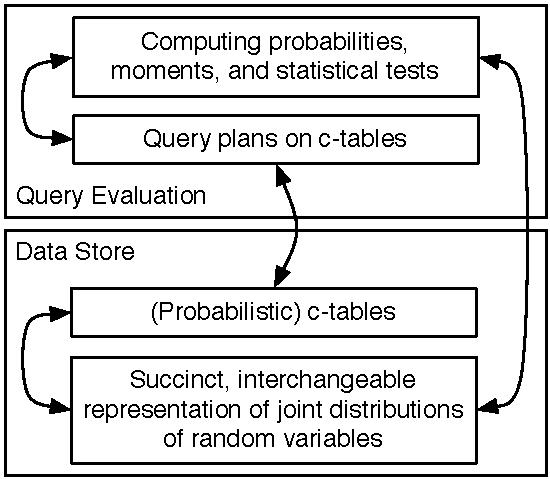
\includegraphics[width=2in]{graphics/arch.pdf}
\vspace*{-0.1in}
\caption{Pip Query Engine Architecture}
\label{fig:arch}
\end{center}
\vspace*{-0.35in}
\end{figure}

\subsection{Symbolic Representation}
PIP represents probabilistic data values symbolically via random variables defined in terms of parametrized probability distribution classes.  PIP supports several generic classes of probability distributions (e.g., Normal, Uniform, Exponential, Poisson), and may be extended with additional classes.  Variables are treated as opaque while they are manipulated by traditional relational operators.  The resulting symbolic representation is a c-table.  As the final stage of the query, special operators defined within PIP compute expectations and moments of the uncertain data, or sample the data to generate histograms.  

These expectation operators are invoked with an unbiased, lossless representation of the expression to be evaluated.  Because the variables have been treated as opaque, the expectation operator can obtain information about the distribution a variable corresponds to.  Developers can (but need not) provide supplemental information (e.g., functions defining the PDF and the CDF) about distributions they extend PIP with.  The operator can exploit this additional information to accelerate the sampling process, or potentially even sidestep it entirely.  For example, if a query asks for the probability that a variable will fall within specified bounds, the expectation operator can compute it with at most two evaluations of the variable's CDF.

Because the symbolic representation PIP uses is lossless, intermediate query results or views may be materialized.  Expectations of values in these views or subsequent queries based on them will not be biased by estimation errors introduced by materializing the view.  This is especially useful when a significant fraction of query processing time is devoted to managing deterministic data (eg, to obtain parameters for the model's variables).  Not only can this accelerate processing of commonly used subqueries, but it makes online sampling feasible; the sampler need not evaluate the entire query from scratch to generate additional samples.

\begin{example}\em
Consider the running example in the context of c-tables. The result of the relational algebra part of the
example query can be easily computed as
\[
\begin{tabular}{c|c|c}
R & Price & Condition \\
\hline
& $X_1$ & $X_2 \ge 7$ \\
\end{tabular}
\]
without looking at $p$.
This c-table compactly represents all data still relevant after the
application of the relational algebra part of the query, other than $p$,
which remains unchanged.
Sampling from R to compute
\begin{verbatim}
select expected_sum(Price) from R;
\end{verbatim}
is a much more focused effort.
First, we only have to consider the random variables relating to Joe;
but determining that random variable $X_2$ is relevant while $X_4$
is not requires
executing a query involving a join. We want to do this query first, before
we start sampling.

Second, assume that delivery times are
independent from sales volumes. Then we can approximate the
query result
by first sampling an $X_2$ value and only sampling an $X_1$ value if $X_2 \ge 7$.
Otherwise, we use $0$ as the $X_1$ value.
If $X_2 \ge 7$ is relatively rare (e.g., the average shipping times to NY are
very slow, with a low variance), this may reduce the amount of samples
for $X_1$ that are first computed and then discarded without seeing use
considerably.
If CDFs are available, we can of course do even better.
%
\end{example}

\subsection{Random Variables}

At the core of PIP's symbolic representation of uncertainty is the random variable, represented in PIP as a 4-tuple.  Each random variable consists of a unique identifier, a subscript (for multi-variate distributions), a distribution class, and a set of parameters for the distribution.  

For example, we write 
$$[X\Rightarrow Normal(\mu,\sigma^2)]$$
 to represent a normally distributed random variable $X$ with mean $\mu$ and standard deviation $\sigma^2$.  Multivariate distributions may be written in the form 
$$[X[n]\Rightarrow MVNormal(\mu, \sigma^2, N)]$$

Thus, when instantiating a random variable, users specify both a distribution for the variable to be sampled from, and a parameter set for that distribution.  As a single variable may appear simultaneously at multiple points within the database, the unique identifier is used to ensure that sampling processes generate consistent values for the variable within a given sample.  

Random variables are stored, either directly or as arithmetic formulas, in the tables of a database.  The equation datatype used for this purpose is simply a flattened parse tree of the formula.  Observe that while we limit our implementation to arithmetic operators, any non-recursive expression may be similarly represented; The equation datatype can potentially be used to encode any target expression accepted by PostgreSQL.  

Random variable equations can be combined freely with constant expressions, both in the target clause of a select statement, and in the where clause.  All targets including random variable equations are encoded as random variable equations themselves.  All where clauses including random variable equations are encoded as c-table conditions.  As this allows a variable to appear several times in a given context, the variable's identifier is used as part of the seed for the pseudorandom number generator used by the sampling processes.

C-table conditions allow PIP to represent per-tuple uncertainty.  Each tuple is tagged with a condition that must hold for the variable to be present in the table.  C-table conditions are expressed as a boolean equation of \textit{atoms}, arbitrary inequalities of random variables.  The independent probability, or \textit{confidence} of the tuple is the probability of the condition being satisfied.  

Given  tables  in which  all  conditions  are  conjunctions of  atomic conditions and  the query does not employ  duplicate elimination, then all conditions  in the output  table are conjunctions.  Thus  it makes sense to particularly optimise this scenario \cite{AJKO2008}. In the case of positive relational algebra  with the duplicate elimination  operator (i.e., we trade  duplicate   elimination  against  difference),   we  can  still efficiently  maintain  the  conditions  in  DNF,  i.e.,  as  a  simple disjunction of conjunctions of atomic conditions.

Without loss of generality, the model can be limited to conditions that are conjunctions of constraint  atoms.  Generality  is maintained by  using bag  semantics to encode disjunctions. This  restriction   provides   several  benefits. First, constraint  validation is  simplified;  A pairwise  comparison of  all atoms in the clause is  sufficient to catch the inconsistencies listed above.   As an additional  benefit, if  all atoms  of a  clause define convex and  contiguous regions in the space $\vec{x},\vec{y}$, these same properties are also shared by their intersection.

\subsection{Condition Inconsistency}
Conditions can become \textit{inconsistent} by combining contradictory conditions using conjunction, which may happen in the implementations of the operators selection, product, and difference.  If such tuples are discovered, they may be freely removed from the c-table.  

A condition is consistent if there is a variable assignment that makes the condition true. For general boolean formulas, deciding consistency is computationally hard. But we do not need to decide it during the evaluation of relational algebra operations.  Rather, we exploit straightforward cases of inconsistency to clean-up c-tables and reduce their sizes. We rely on the later Monte Carlo simulation phase to enforce the remaining inconsistencies.
%
\begin{enumerate}
\item The consistency of conditions not involving variable values is always immediately apparent.
\item Conditions $X_i = c_1 \land X_i = c_2$ with constants $c_1 \neq c_2$ are always inconsistent.
\item Equality conditions over continuous variables $Y_j = (\cdot)$, with the exception of the identity $Y_j = Y_j$, are not inconsistent but can be treated as such (the probability mass will always be zero).  Similarly, conditions $Y_j \neq (\cdot)$, with the exception of $Y_j \neq Y_j$, can be treated as true and removed or ignored.
\item Other forms of inconsistency can also be detected where it is efficient to do so.
\end{enumerate}

With  respect to discrete variables, inconsistency detection may be further simplified.  Rather than using abstract representations, every row containing discrete variables may be exploded into one row for every possible valuation.  Condition atoms matching each variable to its valuation are used to ensure mutual exclusion of each row.  Thus, discrete variable columns may be treated as constants for the purpose of consistency checks.  As shown in \cite{AJKO2008}, deterministic database query optimizers do a satisfactory job of ensuring that constraints over discrete variables are filtered as soon as possible.

%\vspace*{0.05in}
\begin{figure}
\begin{algorithm} Checking the consistency of a condition
\label{alg:consistCheck}
\footnotesize
\begin{enumerate}
\item $consistencyCheck($ConditionSet $C)$
\item \hspace*{0.1in} foreach \textit{Discrete} condition $[X = c_1] \in C$
\item \hspace*{0.2in} if $\exists [X = c_2] \in C$ s.t. $c_1 \neq c_2$, return \textbf{Inconsistent.}
\item \hspace*{0.1in} foreach \textit{Continuous} variable group $K$ (See Section \ref{subsec:samplingTechs})
\item \hspace*{0.2in} initialize map $S_0$ s.t. $S_0[X] = [-\infty,\infty]\ \forall X \in K$
\item \hspace*{0.2in} while $S_{t} \neq S_{t-1}$ (incrementing $t>0$ each iteration)
\item \hspace*{0.3in} let $S_{t} = S_{t-1}$
\item \hspace*{0.3in} foreach equation $E \in K$
\item \hspace*{0.4in} if $\exists$ no more than one $X\in E$ s.t. $S_{t-1}[x] = [-\infty,\infty]$
\item \hspace*{0.5in} foreach $X$, $S_{t}[X] = S_{t-1} \cap tighten_N(X,E,S_{t})$\\ \hspace*{0.7in} (Where $N = $ the degree of E)
\item \hspace*{0.5in} if $tighten_N$ has not been defined, skip $E$.
\item \hspace*{0.3in} if $\exists X$ s.t. $S_{t}[X] = \emptyset$, return \textbf{Inconsistent.}
\item \hspace*{0.1in} if no Eqns were skipped return \textbf{Consistent.} else return \textit{Consistent.}
\end{enumerate}
\begin{enumerate}
\item $tighten_1($Variable $X,$ Equation $E,$ IntervalMap $S)$
\item \hspace*{0.1in} Express E in normal form $aX + bY + cZ + \ldots > 0$
\item \hspace*{0.2in} if $a > 0$, return $[-\max_{S[Y,Z,\ldots]}(bY+cZ+\ldots)/a, \infty]$
\item \hspace*{0.2in} if $a < 0$, return $[-\infty, -\max_{S[Y,Z,\ldots]}(bY+cZ+\ldots)/a]$
\end{enumerate}
\end{algorithm}
{\footnotesize Strong consistency guarantees returned by this algorithm are marked in \textbf{bold}, while weak ones are marked in \textit{italics}.}
\vspace*{-0.2in}
\end{figure}

This sampling algorithm is presented in Algorithm \ref{alg:consistCheck}.  Due to space constraints only $tighten_1$ is presented in this paper, but all polynomial equations may be handled using a similar, albeit more complex enumeration of coefficients\footnote{PIP limits itself to 2nd degree polynomials}.  We have decided to limit PIP to simple algebraic operators in the current implementation, thus all variable expressions are polynomial.  As this process is optional, more complex equations need not be handled by it.

\subsection{Distributions}
As variables are defined in terms of parametrized distribution classes, PIP's infrastructure is agnostic to the implementation of the underlying distributions.  When defining a distribution, programmers need only include a mechanism for sampling from that distribution; much like \cite{MCDB}'s VG Functions.  However, PIP is not limited to simple sampling functionality.  If it is possible to efficiently compute or estimate the distribution's probability density function ($PDF$), cumulative distribution function ($CDF$), and/or inverse cumulative distribution function ($CDF^{-1}$), these may be included to improve PIP's efficiency.  

Distribution specific values like the $PDF$, $CDF$ and inverse $CDF$ are used to demonstrate what can be achieved with PIP's framework.  Further distribution-specific values like weighted-sampling, mean, entropy, and the higher moments can be used by more advanced statistical methods to achieve even better performance.  The process of defining a variable distribution is described further in Section \ref{sec:implementation}.  

Though PIP abstracts the details of a variable's distribution from query evaluation, it distinguishes between discrete and continuous distributions.  As described in Section \ref{sec:background}, existing research into c-tables has demonstrated efficient ways of querying variables sampled from discrete distributions.  PIP employs similar techniques when it is possible to do so.



\section{Implementation}
\label{sec:implementation}
In order to evaluate the viability of PIP's c-tables approach to continuous variables, we have implemented an initial version of PIP as an extension to the PostgreSQL DBMS as shown in Figure \ref{fig:blockdiag}.  %PIP's extended functionality is provided by a set of user-defined functions written in C.  

\begin{figure}
\begin{center}
\resizebox{1.8in}{!}{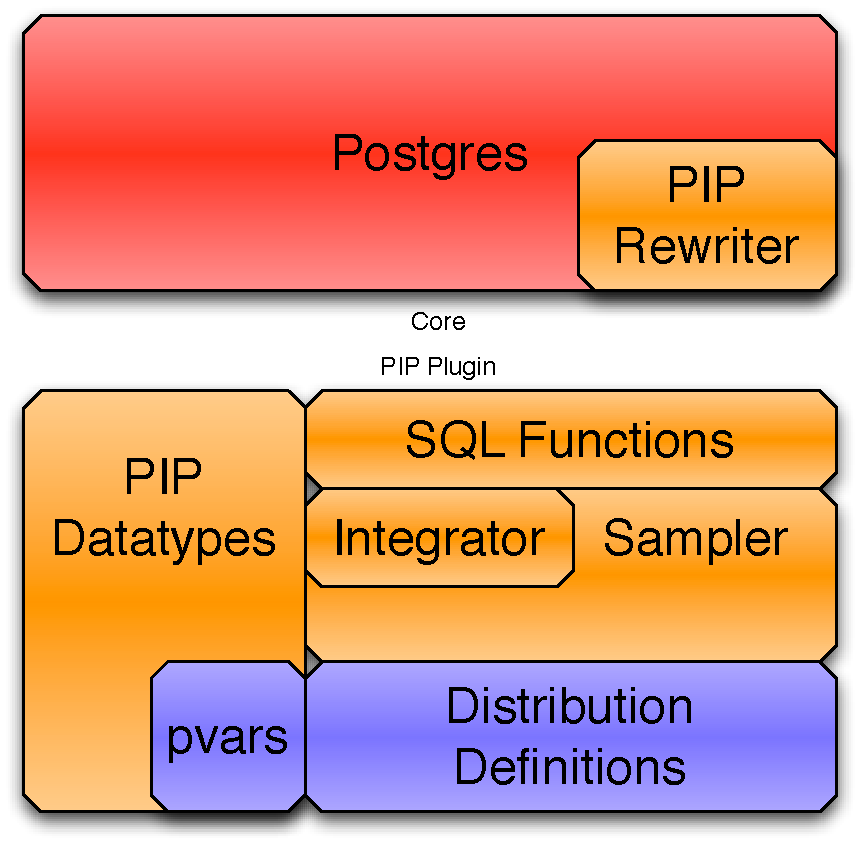
\includegraphics{graphics/blockdiag.pdf}}
\caption{The PIP Postgres plugin architecture}
\label{fig:blockdiag}
\end{center}
\vspace*{-0.3in}
\end{figure}

\subsection{Query Rewriting}
Much of this added functionality takes advantage of PostgreSQL's extensibility features, and can be used ``out-of-the-box".  For example, we define the function \vspace*{-0.1in}
\[
\mbox{\textbf{\footnotesize CREATE\_VARIABLE($distribution$[,$params$])}}\vspace*{-0.1in}
\]
which is used to create continuous variables\footnote{For discrete distributions, PIP uses a repair-key operator similar to that used in \cite{KochMayBMS2008}}.  Each call allocates a new variable, or a set of jointly distributed variables and initializes it with the specified parameters.  When defining selection targets, operator overloading is used to make random variables appear as normal variables; arbitrary equations may be constructed in this way.  

%\begin{example}\em
%Continuous variables may be created inline with the create-variable operation.  
%
%\begin{verbatim}
%select o.order_id, o.item_id,
%       CREATE_VARIABLE (`Normal', p.mean,
%         p.std_dev) AS delivery_time
%from   orders o, params p
%where  o.item_id = p.item_id;
%\end{verbatim}
%
%\end{example}

%Angle brackets around a random variable are shorthand for the variable's expectation.  All instances of this are replaced by a call to pip's expectation sampling function.  

To complete the illusion, we have modified PostgreSQL itself to add support for C-Table constructs.  Under the modified PostgreSQL when defining a datatype, it is possible to declare it as a CTYPE; doing so has the following three effects:
\begin{itemize}
\item CTYPE columns (and conjunctions of CTYPE columns) may appear in the WHERE and HAVING clauses of a SELECT statement.  When found, the CTYPE components of clause are moved to the SELECT's target clause.  For example, if either $(A>B)$ resolves to a CTYPE variable, 
{\small\begin{verbatim}
  select *
  from   inputs
  where  X>Y and Z like '%foo'
\end{verbatim}}
is rewritten to
{\small\begin{verbatim}
  select *, X>Y
  from   inputs
  where  Z like '%foo'
\end{verbatim}}

\item SELECT target clauses are rewritten to ensure that all CTYPE columns in input tables are passed through.   The exception to this is in the case of special probability-removing functions.  If the select statement contains one or more such functions (typically aggregates, or the conf operator), CTYPE columns are not passed through.  

\item In the case of aggregates, the mechanism by which CTYPE columns may be passed through is unclear.  Thus If the select statement contains an aggregate and one or more input tables have CTYPE columns, the query causes an error unless the aggregate is labeled as a probability-removing function.

\item UNION operations are rewritten to ensure that the number of CTYPE columns in their inputs is consistent.  If one input table has more CTYPE columns of a given type than the other, the latter is padded with NULL constraints.

\end{itemize}

\begin{figure}
\begin{center}
\footnotesize
\begin{tabular}{c|ccc}
$R_{ctable}$ & $A$ & $B$ & $\phi$ \\ \hline
& $X*3$ & $5$ & $X > Y \wedge Y > 3$ \\
& $Y$ & $3$ & $Y < 3 \vee X < Y$ \\
\end{tabular}
\begin{center}
$\Downarrow \Downarrow \Downarrow$
\end{center}
\begin{tabular}{c|cccc}
$R_{int}$ & $A$ \begin{footnotesize}(VarExp)\end{footnotesize} & $B$ \begin{footnotesize}(integer)\end{footnotesize} & $\phi_1$ \begin{footnotesize}(CTYPE)\end{footnotesize}& $\phi_2$  \begin{footnotesize}(CTYPE)\end{footnotesize} \\ \hline
& $X*3$ & $5$ & $X > Y$ & $Y > 3$ \\
& $Y$ & $3$ & $Y < 3$ & NULL \\
& $Y$ & $3$ & $X < Y$ & NULL \\
\end{tabular}
\caption{Internal representation of C-Tables}
\label{fig:intrep}
\end{center}
\vspace*{-0.3in}
\end{figure}



Note that these extensions are not required to access PIP's core functionality; they exist to allow users to seamlessly use deterministic queries on probabilistic data.

PIP takes advantage of this by encoding constraint atoms in a CTYPE datatype; Overloaded $>$ and $<$ operators return a constraint atom instead of a boolean if a random variable is involved in the inequality, and the user can ignore the distinction between random variable and constant value (until the final statistical analysis).


\subsection{Defining Distributions}
PIP's primary benefit over other c-tables implementations is its ability to admit variables chosen from arbitrary continuous distributions.  These distributions are specified in terms of general distribution classes, a set of C functions that describes the distribution.  In addition to a small number of functions used to parse and encode parameter strings, each PIP distribution class defines one or more of the following functions.
\begin{itemize}
\footnotesize
\item \texttt{Generate(Parameters, Seed)} uses a pseudorandom number generator to generate a value sampled from the distribution.  The seed value allows PIP to limit the amount of state it needs to maintain; multiple calls to Generate with the same seed value produce the same sample, so only the seed value need be stored.
\item \texttt{PDF(Parameters, x)} evaluates the probability density function of the distribution at the specified point.  
\item \texttt{CDF(Parameters, x)} evaluates the cumulative distribution function at the specified point.
\item \texttt{InverseCDF(Parameters, Value)} evaluates the inverse of the cumulative distribution function at the specified point.
\end{itemize}

PIP requires that all distribution classes define a Generate function.  All other functions are optional, but can be used to improve PIP's performance if provided; The supplemental functions need only be included when known methods exist for evaluating them efficiently.

%Future implementations could conceivably generalize the sampling process.  A sample may be generated using any of the four functions: The Metropolis-Hastings algorithm can sample from an arbitrary PDF, the inverse CDF evaluated on a uniform random value produces a sample, and a binary search may be used to evaluate the inverse CDF given the CDF.

\subsection{Sampling Functionality}
PIP provides several functions for analyzing the uncertainty encoded in a c-table.  The two core analysis functions are conf() and expectation().

\begin{itemize}
\footnotesize
\item \texttt{conf()} performs a conjunctive integration to estimate the probability of a specific row being present in the output, in effect computing the expectation $E[1]$.  It identifies and extracts all lineage atoms from the row being processed and then performs the conjunctive integration over them as normal.

\item \texttt{aconf()}, a variant of conf(), is used to perform general integration.  This function is an aggregate that computes the joint probability of at least one aggregated row being present in the output.  

\item \texttt{expectation()} computes the expectation of a variable by repeated sampling.  If a row is specified when the function is called, the sampling process is constrained by the constraint atoms present in the row.

\item \texttt{expected\_sum()}, \texttt{expected\_max()} are aggregate variants of expectation.  As with expectation() they can be parametrized by a row to specify constraints.

\item \texttt{expected\_sum\_hist()}, \texttt{expected\_max\_hist()} are similar to the above aggregates in that they perform sampling.  However, instead of outputting the average of the results, it instead outputs an array of all the generated samples.  This array may be used to generate histograms and similar visualizations.
\end{itemize}

Aggregates pose a challenge for the query phase of the PIP evaluation process.  Though it is theoretically possible to create composite variables that represent aggregates of their inputs, in practice it is infeasible to do so.  The size of such a composite is not just unbounded, but linear in the size of the input table.  A composite aggregate variable could easily grow to an unmanageable level.  Instead, PIP limits random variable aggregation to the sampling phase.  





\section{Evaluation}
\label{sec:evaluation}


\begin{figure}
\begin{center}
%\input{graphics/scaling_selectivity.tex}
\resizebox{3in}{!}{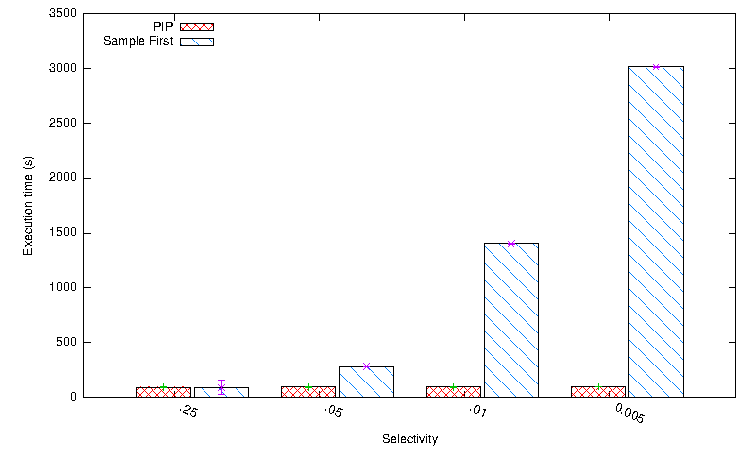
\includegraphics{graphics/scaling_selectivity.pdf}}
\caption{Time to complete a 1000 sample query, accounting for selectivity-induced loss of accuracy.}
\label{fig:scaling_selectivity}
\end{center}
\vspace*{-0.3in}
\end{figure}


\begin{figure}
\begin{center}
\resizebox{3in}{!}{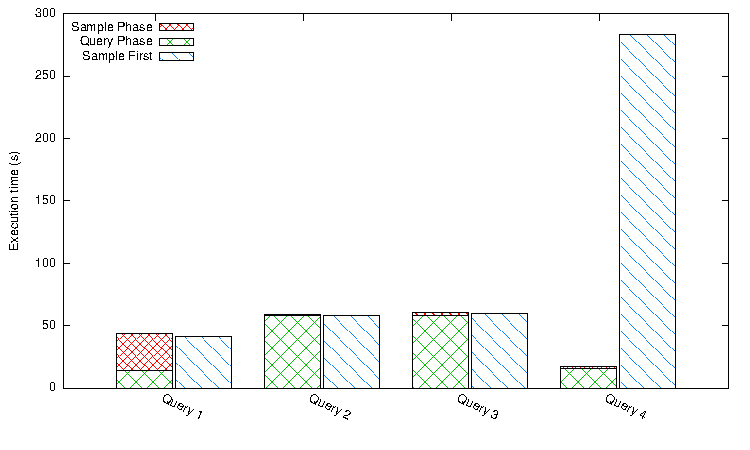
\includegraphics{graphics/query_timings.pdf}}
\caption{Query evaluation times in PIP and Sample-First for a range of queries.  Sample-First's sample-count has been adjusted to match PIP's accuracy.}
\label{fig:querytimings}
\end{center}
\vspace*{-0.3in}
\end{figure}

\begin{figure*}
\begin{center}
\subtable[]{\resizebox{3in}{!}{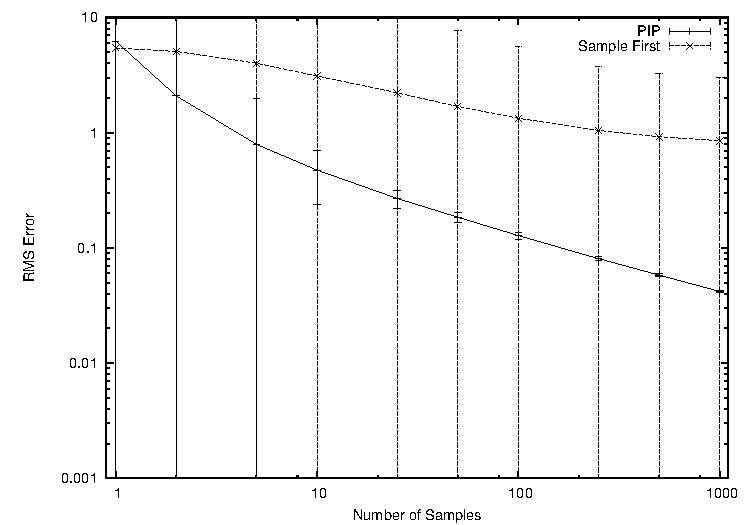
\includegraphics{graphics/variance.pdf}} \label{subfig:variance1}}
\subtable[]{\resizebox{3in}{!}{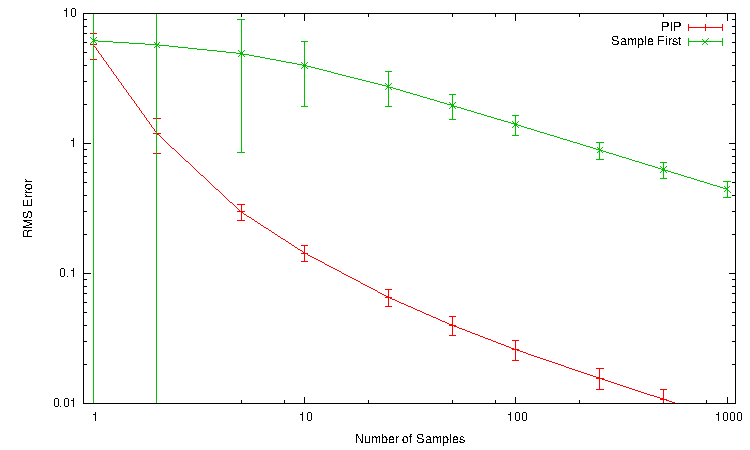
\includegraphics{graphics/variance2.pdf}}\label{subfig:variance2}}
\vspace*{-0.1in}
\caption{RMS error across the results of 30 trials of (a) a simple group-by query $Q_4$ with a selectivity of $0.005$, and (b) a complex selection query $Q_5$ with an average selectivity of $0.05$.}
\label{fig:variance}
\end{center}
\vspace*{-0.3in}
\end{figure*}

As a comparison point for PIP's ability to manage continuous random variables, we have constructed a sample-first probabilistic extension to Postgres that emulates MCDB's tuple-bundle concept using ordinary Postgres rows.  A sampled variable is represented using an array of floats, while the tuple bundle's presence in each sampled world is represented using a densely packed array of booleans.  In lieu of an optimizer, test queries were constructed by hand so as to minimize the lifespan of either array type.

Using Postgres as a basis for both implementations places them on an equal footing with respect to DBMS optimizations unrelated to probabilistic data.  This makes it possible to focus our comparison solely on the new, probabilistic functionality of both systems.  However, to make the distinction from MCDB (which is a separate development not based on Postgres) explicit, we refer to our implementation of the MCDB approach as Sample-First.

We evaluated both the PIP C-Tables and the Sample-First infrastructure against a variety of related queries.  Tests were run over a single connection to a modified instance of PostgreSQL 8.3.4 with default settings running on a 2x4 core 2.0 GHz Intel Xeon with a 4MB cache.  Unless otherwise specified queries were evaluated over a 1 GB database generated by the TPC-H benchmark, all sampling processes generate 1000 samples apiece, and results shown are the average of 10 sequential trials with error bars indicating one standard deviation.

First, we demonstrate PIP's performance on a simple set of queries ideally suited to the strengths of Sample-First.  These two queries (identical to Q1 and Q2 from \cite{MCDB}) involve pa\-ra\-me\-tri\-zing a table of random values, applying a simple set of math operations to the values, and finally estimating the sum of a large aggregate over the table.  

The first query computes the rate at which customer purchases have increased over the past two years.  The percent increase parametrizes a Poisson distribution that is used to predict how much more each customer will purchase in the coming year.  Given this predicted increase in purchasing, the query estimates the company's increased revenue for the coming year.

In the second query, past orders are used to compute the mean and standard deviation of manufacturing and shipping times.  These values parametrize a pair of Normal distributions that combine to predict delivery dates for each part ordered today from a Japanese supplier.  Finally, the query computes the maximum of these dates, providing the customer with an estimate of how long it will take to have all of their parts delivered.

The results of these tests are shown as query $Q_1$ and $Q_2$, respectively, in Figure \ref{fig:querytimings}.  Note that performance times for PIP are divided into two components: query and sample, to distinguish between time spent evaluating the deterministic components of a query and building the result c-table, and time spent computing expectations and confidences of the results.  The results are positive; the overhead of the added infrastructure is minimal, even on queries where Sample-First is sufficient.  Furthermore, especially in Q2, the sampling process comprises a relatively small portion of the query; additional samples can be generated without incurring the nearly 1 minute query time.

The third query $Q_3$ in Figure \ref{fig:querytimings} combines a simplified form of queries $Q_1$ and $Q_2$.  Rather than aggregating, the query compares the delivery times of $Q_2$ to a set of ``satisfaction thresholds."  This comparison results in a (probabilistic) table of dissatisfied customers that is used in conjunction with $Q_1$'s profit expectations to estimate profit lost to dissatisfied customers.  A query of this form might be run on a regular basis, perhaps even daily.  As per this usage pattern, we pre-materialize the component of this query unlikely to change on a daily basis: the expected shipping time parameters.

%  $Q_3$ is described in more detail in the Appendix Section \ref{sec:timingq3}

Though PIP and Sample-First both take the same amount of time to generate 1000 samples under this query, the query's selectivity causes Sample-First to disregard a significant fraction of the samples generated; for the same amount of work, Sample-First generates a less accurate answer.  To illustrate this point, see Figure \ref{subfig:variance1}.  This figure shows the RMS error, normalized by the correct value in the results of a query for predicted sales of 5000 parts in the database, given a Poisson distribution for the increase in sales and a popularity multiplier chosen from an exponential distribution.  As an additional restriction, the query considers only the extreme scenario where the given product has become extremely popular (resulting in a selectivity of $e^{-5.29} \approx 0.005$).  

RMS error was computed over 30 trials using the algebraically computed correct value as a mean, and then averaged over all 5000 parts.  Note that PIP's error is over two orders of magnitude lower than the sample-first approach for a comparable number of samples.  This corresponds to the selectivity of the query; as the query becomes more selective, the sample-first error increases.  Furthermore, because CDF sampling is used to restrict the sampling bounds, the time taken by both approaches to compute the same number of samples is equivalent.

A similar example is shown in Figure \ref{subfig:variance2}.  Here, a model is constructed for how much product suppliers are likely to be able to produce in the coming year based on an Exponential distribution, and for how much product the company expects to sell in the coming year as in Q1.  From this model, the expected underproduction is computed, with a lower bound of 0; the selection criterion considers only those worlds where demand exceeds supply.  For the purposes of this test, the model was chosen to generate an average selectivity of 0.05.  Though the comparison of 2 random variables necessitates the use of rejection sampling and increases the time PIP spends generating samples, the decision to drop a sample is made immediately after generating it; PIP can continue generating samples until it has a sufficient number, while the Sample-First approach must rerun the entire query.

Note the relatively large variance in the RMS error of the Sample-First results these figures, particularly the first one.  Here, both the selectivity and the price for each part vary with the part.   Thus, some parts become more important while others become harder to sample from.  In order to get a consistent answer for the entire query Sample-First must provision enough samples for the worst case, while PIP can dynamically scale the number of samples required for each term.

Returning to Figure \ref{fig:querytimings}, Queries $Q_3$ and $Q_4$ have been run with PIP at a fixed 1000 samples.  As Sample-First drops all but a number of samples corresponding to the selectivity of the query, we run Sample-First with a correspondingly larger number of samples.  For Query 3, the average selectivity of 0.1 resulted in Sample-First discarding 10\% of its samples.  To maintain comparable accuracies, Sample-First was run at 10,000 samples.  

We expand on this datapoint in Figure \ref{fig:scaling_selectivity} where we evaluate $Q_4$, altered to have varying selectivities.  The sample-first tests are run with $\frac{1}{selectivity}$ times as many samples as PIP to compensate for the lower error, in accordance with Figure \ref{subfig:variance1}.  Note that selectivity is a factor that a user must be aware of when constructing a query with sample-first while PIP is able to account for selectivity automatically, even if rejection sampling is required.

It should also be noted that both of these queries include two distinct, independent variables involved in the expectation computation.  A studious user may note this fact and hand optimize the query to compute these values independently.  However, without this optimization, a sample-first approach will generate one pair of values for each customer for each world.  As shown in the RMS error example, an arbitrarily large number of customer revenue values will be discarded and the query result will suffer.  In this test, customer satisfaction thresholds were set such that an average of 10\% of customers were dissatisfied.  Consequently sample-first discarded an average of 10\% of its values.  To maintain comparable accuracies, the sample-first query was evaluated with 10,000 samples while the PIP query remained at 1000 samples. 

As a final test, we evaluated both PIP and our Sample-First implementation on the NSIDC's Iceberg Sighting Database\cite{iceberg} for the past 4 years.  100 virtual ships were placed at random locations in the North Atlantic, and each ship's location was evaluated for its proximity to potential threats; Each iceberg in the database was assigned a normally distributed position relative to its last sighting, and an exponentially decaying danger level based on time since last sighting.  Recently sighted icebergs constituted a high threat, while historic sightings represented potential new iceberg locations.  The query identified icebergs with greater than a 0.1\% chance of being located near the ship and estimated the total thret posed by all potentially nearby icebergs.  The results of this experiment are shown in Figure \ref{fig:iceberg}.  PIP was able to employ CDF sampling and obtain an exact result within 10 seconds.  By comparison, the Sample-First implementation generating 10,000 samples took over 10 minutes and produced results deviating by as much as 25\% from the correct result on average.

\begin{figure}
\begin{center}
%\input{graphics/iceberg_danger.tex}
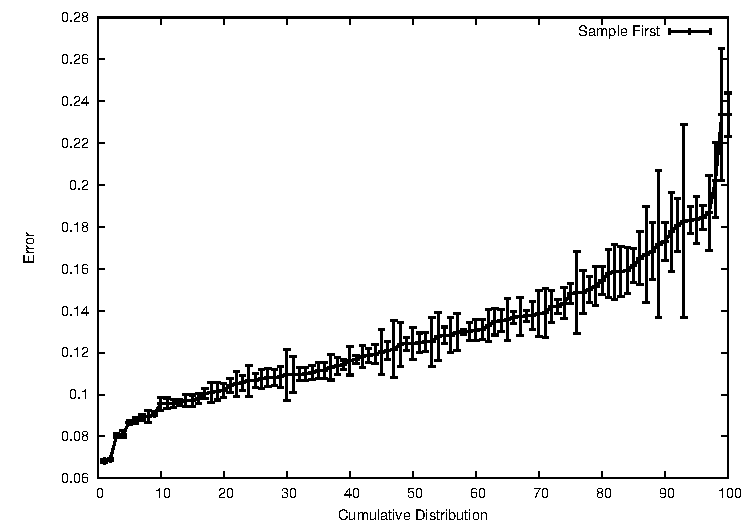
\includegraphics[width=3in]{graphics/iceberg_danger.pdf}
\caption{Sample-First error as a fraction of the correct result in a danger-estimation query on the NSIDC's Iceberg Sighting Database.  PIP was able to obtain an exact result.}
\end{center}
\label{fig:iceberg}
\vspace*{-0.3in}
\end{figure}

%\begin{figure}
%\begin{center}
%\resizebox{3in}{!}{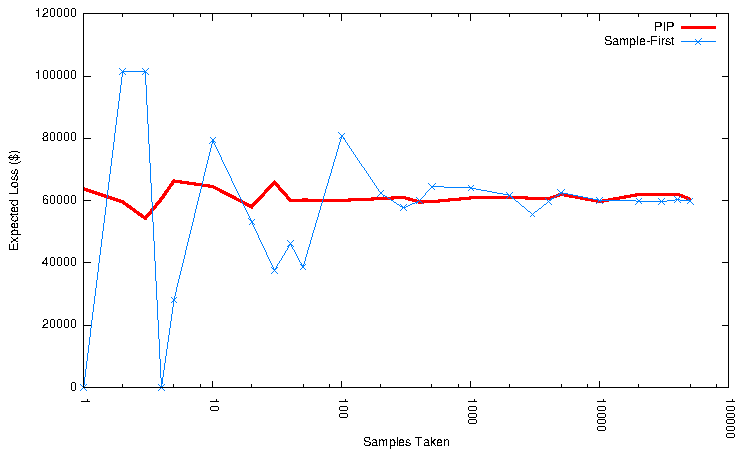
\includegraphics{graphics/iterative_refinement.pdf}}
%\caption{Variance as a function of samples in PIP and Sample-First.  Each data point is an estimate generated by a single run at the indicated number of samples}
%\label{fig:iterativerefinement}
%\end{center}
%\end{figure}
%
%
%Figure \ref{fig:iterativerefinement} demonstrates one extreme case of this in a comparison between Karp-Luby estimates and Sample-First estimates.  The results shown are for repeated executions of a query similar to query 4, save with a filter that removes all but approximately 10 clients.  In queries that do not involve a large linear aggregate, the sample-first approach disqualifies a sufficient number of possible worlds that subsequent expectation computations falter.  Conversely the Karp-Luby estimator has sufficient information that it can employ a precomputed CDF lookup table to compute each row's bag probabilities.  Because of this and the fact that it generates more ``useful'' samples, its results have a much lower variance with far fewer samples required.



\begin{small}
\bibliographystyle{abbrv}
\bibliography{bibtex}
\end{small}


\end{document}
